\chapter{Meccanica del Robot}
Il robot � costituito da tre diverse parti funzionali: una base dotata di ruote motrici,
 un braccio rotante ed un sistema di leve a forbice.

\section{La base}
La base del robot � stata costruita partendo da un modello presente sul sito
della Lego 
(\emph{http://www.active-robots.com/products/mindstorms4schools/building-\\instructions/Build-RoboArm.pdf} Figura \ref{Base})
e modificato come segue: il motore B, che nello schema originale si occupava di
far ruotare il braccio, continua nella sua funzione mentre il motore A
trasferisce la sua funzione da far muovere in avanti il braccio a gestire la trazione del robot.\\

\begin{figure}[h]
\begin{center}
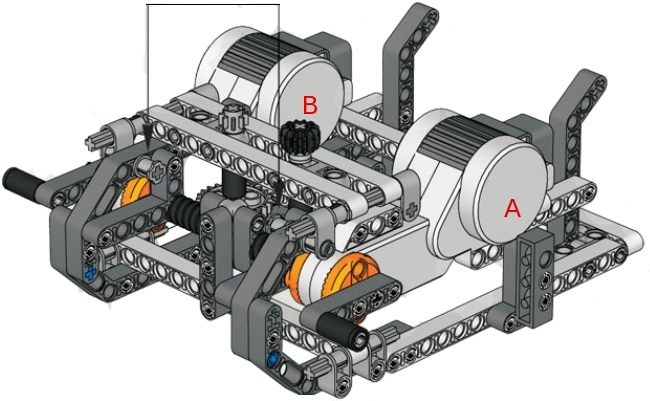
\includegraphics[scale=0.5]{img/base.png}
\caption{Struttura iniziale della Base \label{Base}}
\end{center}
\end{figure}

Per permettere al robot di avanzare, la base � stata montata su quattro ruote di
cui le due anteriori sono le ruote motrici. Quest'ultime sono collegate tra di
loro con un asse motore comune, che riceve il movimento tramite un gioco di
ingranaggi conici trasformando la rotazione dall'asse veticale, prodotta dal
motore A pi� la vite archimedea, in un movimento sull'asse orizzontale
necessario per l'avanzamento del robot.\\

Per cercare di ridurre i giochi meccanici introdotti dal sistema di riduzioni
meccaniche si sono inoltre aggiunte delle parte non originali della Lego. 
 
 
